\part{Caso práctico - Detección de Matrículas}
\section{Contexto y herramientas utilizadas}
Para complementar este trabajo, vamos a crear un programa en \mintinline{python}{Python} que sea capaz de detectar matrículas. Para ello, realizaremos un procesamiento de imágenes de coches para tratar de identificar y dejar claro el recuadro de la matrícula; esto lo haremos con las librerías \mintinline{python}{cv2} \cite{cv2} y \mintinline{python}{skimage} \cite{skimage}. Luego, pasaremos esa imagen por un motor OCR, dado por la librería \mintinline{python}{pytesseract} \cite{pytesseract}.

\section{Características de las imágenes del dataset}
Nuestro dataset está compuesto por 10 imágenes a color cuadradas de 512x512 donde podemos visualizar una matrícula de un coche. Trabajaremos con la imagen \ref{coche1} del dataset:

\begin{figure}[H]
    \centering
    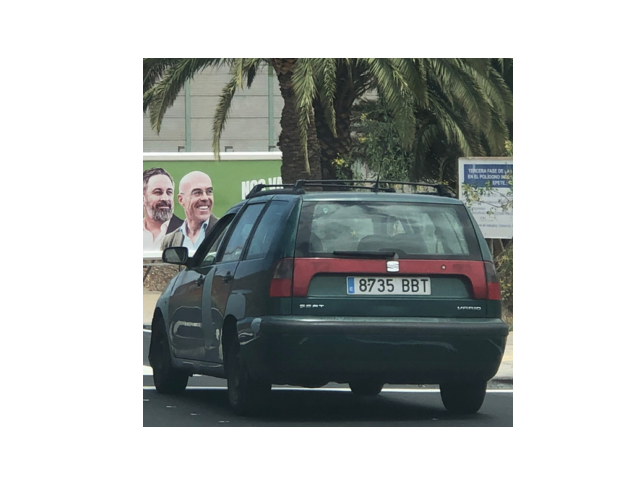
\includegraphics[width=0.6\linewidth]{Images/coche1.png}
    \caption{Imagen de un coche}
    \label{coche1}
\end{figure}

Para cargar esta imagen en el programa, usamos la función:
\begin{minted}{python}
img = cv2.imread("./dataset/coche1.png")
\end{minted}

Para mostrar información de la imagen, usamos:
\begin{minted}{python}
>>> print(img.shape)
(512, 512, 3)
\end{minted}

Esto nos dice que la imagen tiene 512 píxeles de alto, 512 de alto y 3 canales (correspondientes a los colores rojo, verde y azul). 
\begin{figure}[H]
    \centering
    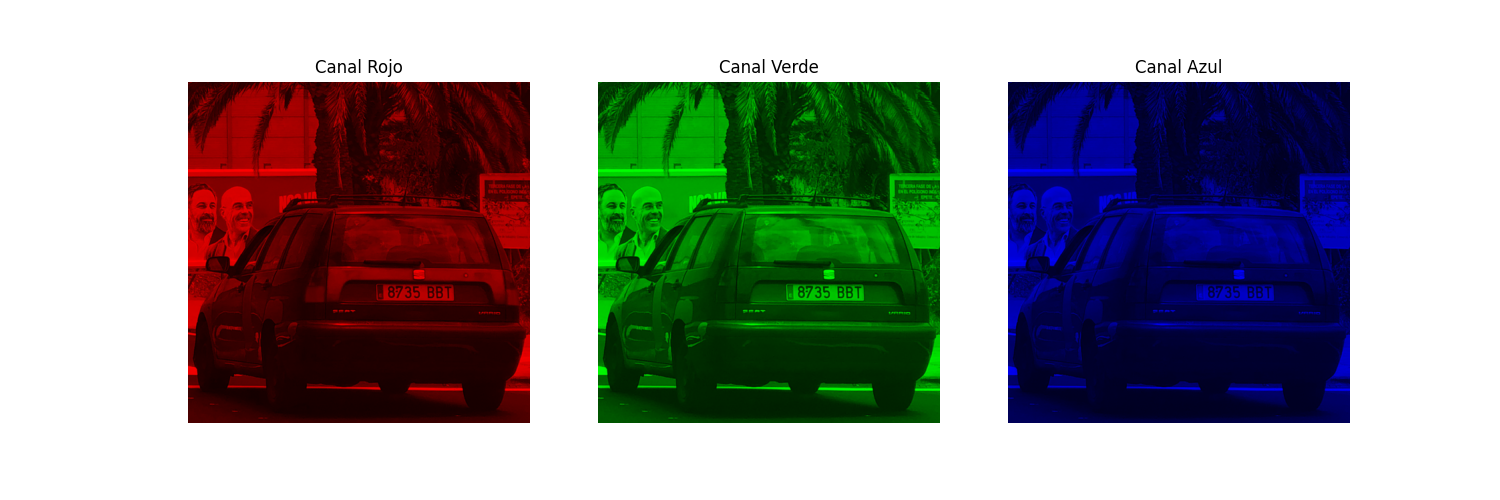
\includegraphics[width=1\linewidth]{Images/coche1Canales.png}
    \caption{3 canales de color}
    \label{coche1Canales}
\end{figure}

\section{Imagen en escala de grises}
Para procesar esta imagen, nos interesa que esta tenga 1 solo canal, es decir, que esté en escala de grises. Para ello, podemos usar:
\begin{minted}{python}
imgBW = cv2.cvtColor(img, cv2.COLOR_BGR2GRAY)
\end{minted}
Obteniendo como resultado la imagen \ref{coche1B&W}:
\begin{figure}[H]
    \centering
    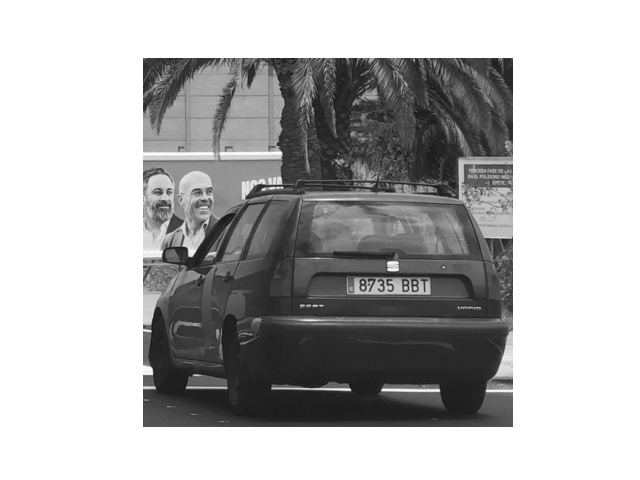
\includegraphics[width=0.6\linewidth]{Images/coche1B&W.png}
    \caption{Coche en escala de grises}
    \label{coche1B&W}
\end{figure}
Comprobemos los detalles de la nueva imagen:
\begin{minted}{python}
>>> print(imgBW.shape)
(512, 512)
\end{minted}
Ahora tenemos 1 solo canal en la imagen.

\section{Imagen binaria}
El siguiente paso sería aplicarle un umbral a la imagen en escala de grises, para que, las matrículas, que son caracteres negros sobre un fondo blanco, queden marcadas y podamos detectar su contorno más fácilmente. La biblioteca \mintinline{python}{cv2} nos ofrece 2 alternativas:
\begin{minted}{python}
value = 170
imgBIN1 = cv2.threshold(imgBW, value, 255, cv2.THRESH_BINARY_INV)[1]
\end{minted}
\begin{minted}{python}
imgBIN2 = cv2.adaptiveThreshold(imgBW, 255, cv2.ADAPTIVE_THRESH_GAUSSIAN_C, 
                    cv2.THRESH_BINARY_INV, 9, 7)
\end{minted}

\mintinline{python}{cv2.threshold} utiliza un umbral global fijo para toda la imagen, es adecuado para imágenes con iluminación uniforme es más rápido y es computacionalmente menos costoso.

En cambio, \mintinline{python}{cv2.adaptativeThreshold} utiliza un umbral que varía localmente según la región de la imagen, es más robusto para imágenes con variaciones de iluminación y es más lento debido al cálculo local del umbral.

\begin{figure}[H]
    \centering
    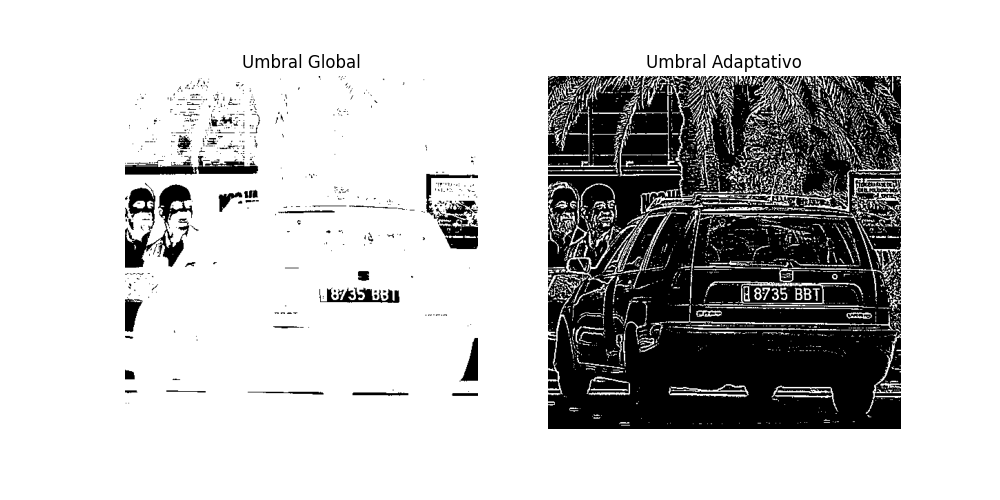
\includegraphics[width=.8\linewidth]{Images/coche1Umbrealizaciones.png}
    \caption{Umbral global y adaptativo}
    \label{coche1Umbrealizaciones}
\end{figure}

Como podemos observar, en ambos casos la matrícula queda bien marcada. En nuestro caso, usaremos \mintinline{python}{cv2.adaptativeThreshold}, que es con el que mejor resultados obtenemos.

\section{Contornos}
Ahora tenemos que encontrar los contornos de la imagen, que son curvas que unen todos los puntos continuos a lo largo de un límite, que tienen el mismo color o intensidad. Esto lo podemos realizar con:
\begin{minted}{python}
contornos = cv2.findContours(imgBIN, cv2.RETR_LIST, cv2.CHAIN_APPROX_SIMPLE)[0]
\end{minted}

Al aplicar esa función a la imagen binaria, obtenemos la imagen \ref{coche1Contornos}:
\begin{figure}[H]
    \centering
    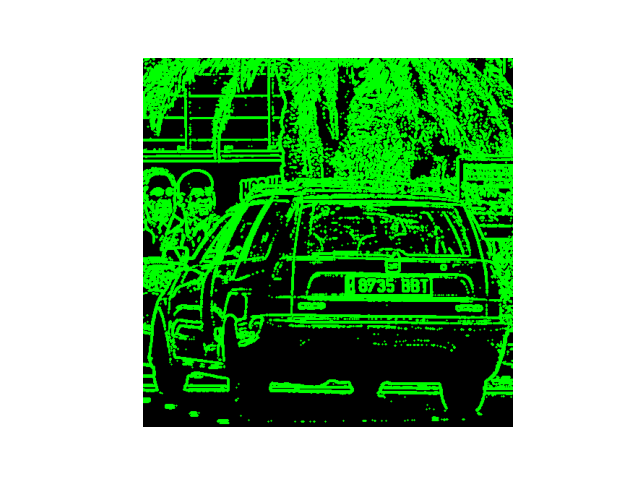
\includegraphics[width=.6\linewidth]{Images/coche1Contornos.png}
    \caption{Contornos del coche}
    \label{coche1Contornos}
\end{figure}

\subsection{Filtrar Contornos}
Para filtrar los contornos primero tenemos que saber cuales son las medidas de las matrículas europeas, que son de 520mm x 120mm. A partir de ahí calculamos la relación de aspecto, que no es más que dividir 520 entre 120. También hemos añadido límites de ancho y alto para evitar que aparezcan contornos muy pequeños o muy grandes.

Entonces, iteramos sobre los contornos que hemos calculado antes y calculamos su relación de aspecto vemos si es parecida a la nuestra. También comprobamos que no sea ni inferior ni superior a los límites establecidos.

\newpage

\begin{minted}{python}
ratio = 520.0/120.0 
min_w = 64
max_w = 256
min_h = 16
max_h = 64
candidatos = []
    for c in contornos:
        x, y, w, h = cv2.boundingRect(c)
        aspect_ratio = float(w) / h

        if (np.isclose(aspect_ratio, ratio, atol=1.5) and
           (max_w > w > .min_w) and
           (max_h > h > min_h)):
                candidatos.append(c)
\end{minted}

En nuestro caso, obtenemos el siguiente candidato \ref{coche1FiltroContorno}, que se corresponde con el contorno de la matrícula del coche:
\begin{figure}[H]
    \centering
    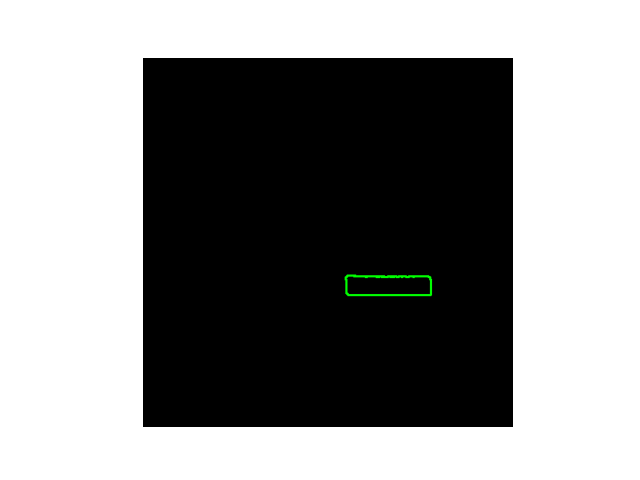
\includegraphics[width=.6\linewidth]{Images/coche1FiltroContorno.png}
    \caption{Contorno filtrado}
    \label{coche1FiltroContorno}
\end{figure}

\subsection{¿Qué ocurre si hay más de un candidato?}
Ha habido coches donde el algoritmo nos ha detectado más de un candidato, bien porque la forma sea similar o bien porque el algoritmo no sea lo suficientemente restrictivo.

En este caso lo que se nos ha ocurrido es seleccionar el candidato más bajo, ya que las matrículas se suelen encontrar en la parte de abajo. 

Esto no es lo más preciso y en otros casos puede fallar. Para mejorar esto se podría intentar perfeccionar el filtrado o dejar que la red neuronal se encargue de seleccionar el mejor candidato.
\begin{minted}{python}
ys = [cv2.boundingRect(c)[1] for c in candidatos]
candidatoMenor = candidatos[np.argmax(ys)]
\end{minted}
En la imagen \ref{coche7Filtrado} tenemos un ejemplo de este suceso:
\begin{figure}[H]
    \centering
    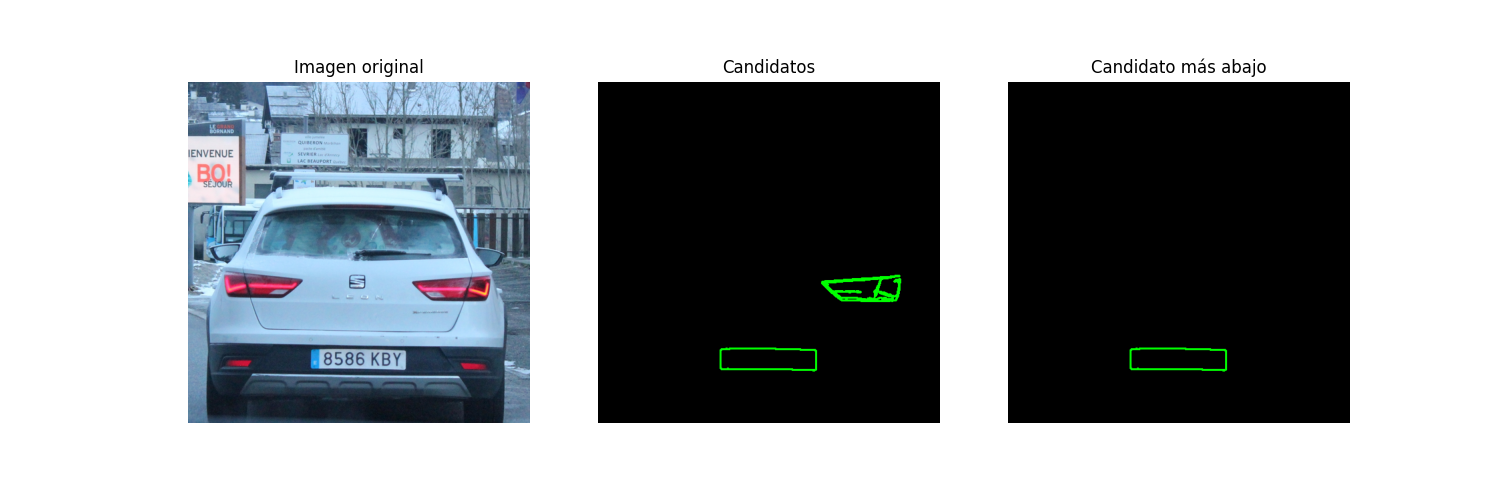
\includegraphics[width=1\linewidth]{Images/coche7Filtrado.png}
    \caption{Varios candidatos}
    \label{coche7Filtrado}
\end{figure}


\section{Recortar matrícula}
En el siguiente paso, tenemos que recortar la parte de la matrícula con ayuda del contorno obtenido, para ello, podemos usar:
\begin{minted}{python}
x, y, w, h = cv2.boundingRect(candidatoMenor)
matricula = img[y:y+h,x:x+w]
\end{minted}
Al aplicar esa función obtenemos la imagen \ref{coche1Matricula}:
\begin{figure}[H]
    \centering
    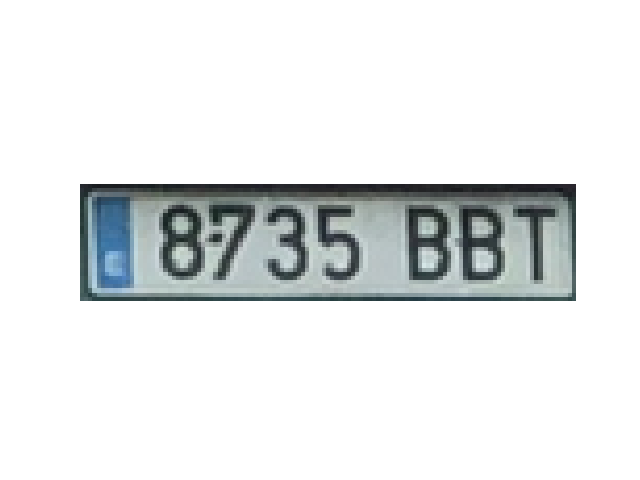
\includegraphics[width=.4\linewidth]{Images/coche1Matricula.png}
    \caption{Matrícula}
    \label{coche1Matricula}
\end{figure}

\section{Procesar matrícula}
Al igual que hicimos con el coche, tenemos que pasar la imagen de la matrícula a blanco y negro para posteriormente binarizarla.
\begin{figure}[H]
    \centering
    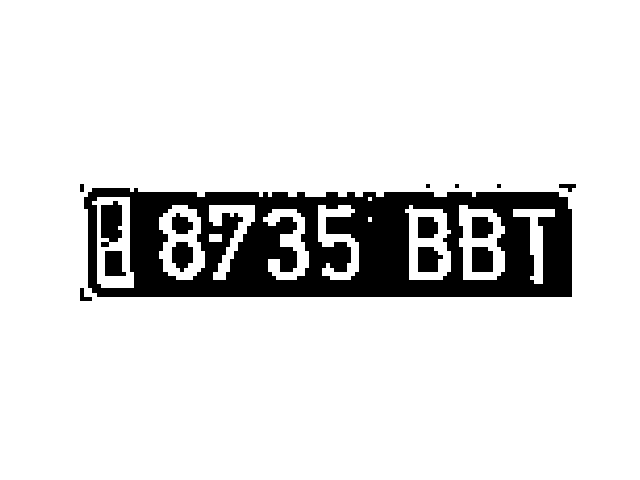
\includegraphics[width=.4\linewidth]{Images/coche1MatriculaUmbral.png}
    \caption{Matrícula binarizada}
    \label{coche1MatriculaUmbral}
\end{figure}

El resultado de la binarización puede ser tener un poco de ruido en los bordes, así que utilizamos una función de \mintinline{python}{skimage} para eliminarlos:
\begin{minted}{python}
matriculaSinBordes = skimage.segmentation.clear_border(matriculaBIN)
\end{minted}

Obtenemos como resultado la imagen \ref{coche1MatriculaSinBordes}:
\begin{figure}[H]
    \centering
    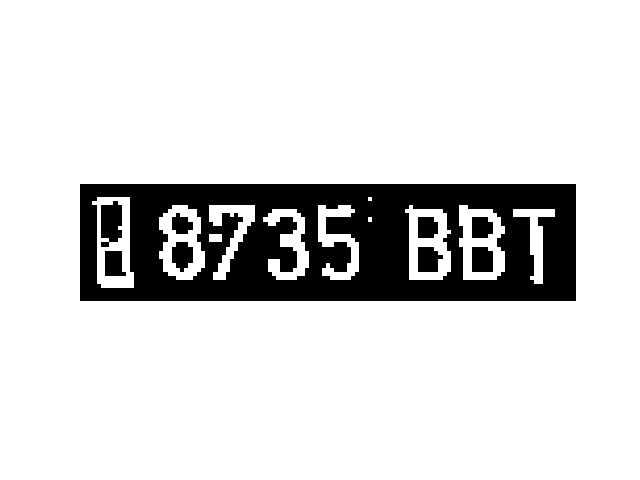
\includegraphics[width=.4\linewidth]{Images/coche1MatriculaSinBordes.png}
    \caption{Matrícula sin ruido en los bordes}
    \label{coche1MatriculaSinBordes}
\end{figure}

Ahora tenemos que invertir la imagen para que \mintinline{python}{pytesseract} la pueda analizar correctamente:
\begin{minted}{python}
matriculaFinal = cv2.bitwise_not(img)
\end{minted}

La imagen \ref{coche1MatriculaFinal} es el resultado final del procesamiento para poder leer matrículas:
\begin{figure}[H]
    \centering
    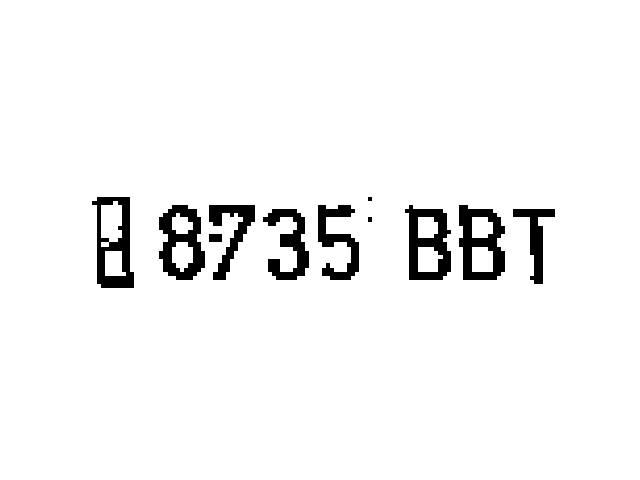
\includegraphics[width=.4\linewidth]{Images/coche1MatriculaFinal.png}
    \caption{Matrícula invertida. Resultado final.}
    \label{coche1MatriculaFinal}
\end{figure}

\section{Extracción del texto}
El primer paso es configurar \mintinline{python}{pytesseract} para que solo nos reconozca las letras y números que contienen la matrícula europea y no nos detecte cualquier otro símbolo. En este caso, queremos reconozca todas las letras excepto las vocales, la \textit{Ñ} y la \textit{Q}; y todos los números:
\begin{minted}{python}
alphanumeric = "BCDFGHJKLMNPRSTVWXYZ0123456789"
options = f"-c tessedit_char_whitelist={alphanumeric} -- psm 7"
txt = pytesseract.image_to_string(img, config=options)
\end{minted}

Las matrículas a reconocer tienen un símbolo a la derecha de la unión europea, el cual \mintinline{python}{pytesseract} puede detectar como quiera. Entonces, la estrategia para devolver la cadena referente a la matrícula será recorrernos la variable \mintinline{python}{txt} a la inversa, para así detectar las 3 primeras letras que aparezcan y los primeros 4 números que siguen a dichas letras. En el caso que no detectemos todos los números o todas las letras, completamos con \textit{?}.
\begin{minted}{python}
txt = txt[::-1]
letras = ""
numeros = ""
counter = 0
for t in txt:
    if ((t in "BCDFGHJKLMNPRSTVWXYZ") and (counter < 3)):
        letras += t
        counter += 1
    if ((t in "0123456789") and (3 <= counter < 7)):
        numeros += t
        counter += 1

letras += "?"*(3 - len(letras)) 
numeros += "?"*(4 - len(numeros)) 
        
matricula = numeros[::-1] + " " + letras[::-1]
\end{minted}

En el caso de ejemplo, la matrícula que reconoce es: \mintinline{python}{8586 KBY}, que se corresponde con la del coche de la imagen \ref{coche1}.

\section{Resultados y conclusiones}
Hemos realizado unas pruebas con un dataset de 10 imágenes de coches y estos son los resultados:
\begin{minted}{python}
ORIGINAL ----  RESULT  ----- SIMILITUD(%)
8735 BBT ---- 8735 BBT ----- 100.0%
7206 KDF ---- 7206 KDF ----- 100.0%
5683 JZG ---- 5533 JZC ----- 62.5%
4386 LJP ---- ?385 LJP ----- 75.0%
4991 KXN ---- ?991 KXN ----- 87.5%
9723 LCP ---- 9723 LCP ----- 100.0%
8586 KBY ---- 8586 KBY ----- 100.0%
8206 MCS ---- 8206 MCS ----- 100.0%
0378 LKF ---- 0373 LKF ----- 87.5%
0798 MNC ---- 0798 MNC ----- 100.0%

Coches totales:               10
Numero de aciertos:           6
Numero de fallos:             4
Porcentaje simbolos erroneos: 8.75%
\end{minted}

Los resultados son bastante buenos, ha habido 6 casos donde ha hallado la matrícula correctamente, 2 casos donde ha fallado por un símbolo y otros 2 casos donde ha fallado por más de 1 símbolos.

En todos los casos ha sido capaz de distinguir la forma de la matrícula, por lo que los fallos se encuentran en la extracción del texto. Vemos que confunde algunos \textit{8} con \textit{3}, el número \textit{4} con la letra \textit{A}, la \textit{G} con la \textit{C},... En resumen, confunde caracteres similares. Esto puede deberse al tipo de fuente de las matrículas (con la cual \mintinline{python}{pytesseract} no está entrenado) y a que \mintinline{python}{pytesseract} no sabe el formato que tiene que reconocer y nos devuelve un string de todo lo que ve; si supiese que los 4 primeros símbolos son números, entonces no confundiría el \textit{4} con la \textit{A}.

Una posible solución sería entrenar un modelo propio que detecte perfectamente la tipografía y la estructura de las matrículas europeas o tratar de minimizar aun más el ruido de la imagen a partir de la cual se hace la extracción y partirla en 2 partes, la primera con solo números y la segunda con solo letras.